\documentclass[11pt]{article}
\usepackage[margin=0.95in]{geometry}
\usepackage{amsmath,amssymb,amsthm}
\usepackage{booktabs}
\usepackage{tikz}
\usepackage{pgfplots}
\pgfplotsset{compat=1.18}
\usepackage{hyperref}
\usepackage[protrusion=true,expansion=false]{microtype}
\hypersetup{hidelinks}

\newtheorem{definition}{Definition}
\newtheorem{theorem}{Theorem}
\newtheorem{lemma}{Lemma}
\newtheorem{corollary}{Corollary}

\newcommand{\sig}{\operatorname{sig}}
\newcommand{\Indist}{\approx_{V}}
\newcommand{\Def}{\mathrm{Def}}
\newcommand{\Vocab}{\mathcal{V}}
\newcommand{\dom}{\mathcal{X}}
\newcommand{\Epos}{E^{+}}
\newcommand{\Eneg}{E^{-}}

\title{Vocabulary Before Search:\\ Query-Driven Representation Change for Concept Discovery}
\author{}
\date{Draft---\today}

\begin{document}
\maketitle

\begin{abstract}
Recovering an unstated concept $S$ from a handful of examples is a core inductive task, yet concept
analysis, logic programming and program induction all search \emph{within} a given representation
language. No criterion decides when the representation, not the search, is what must change. We show
that when a positive and a negative example are indistinguishable under the vocabulary, no expressible
hypothesis is consistent, and further examples only add constraints; the question shifts from how to
search to which predicate to add, and at what cost. We type that step: five classes of operator
(generation, closure, representation change, evidence, control) share one state and one measure, the
number of live hypotheses, and four theorems fix what each can change, so representation change and
evidence must alternate. Proposal becomes a covering problem, where greedy lands within about $15\%$ of
the optimum. We give an exploration procedure in which a model proposes predicates, a program asks about
representatives of unresolved classes, and an oracle adjudicates, reliable up to about $20\%$
per-answer error. Two negative results bound the design space: object-level query selection is second
order, and adaptive noise gates lose to fixed margins. Total cost follows $r/q$ plus the query rounds,
and the core statements are mechanized in Lean~4; as proposals become cheap, the cost tends to the
rounds, so cheap proposals buy a better vocabulary, not fewer questions.
\end{abstract}

\section{Introduction}

Induction from finitely many examples has two familiar failure modes: the search does not reach the
target, or the background knowledge does not contain the pattern. A third failure is logical rather
than computational. The target concept may fail to be expressible over the vocabulary the search
ranges over; the hypothesis space then holds no consistent element, and no amount of search inside a
language produces a sentence outside it. The failure looks like weak evidence, and it is usually
reported as weak evidence, although no further example can remove it.

\textbf{Contributions.} We give a decidable criterion for an insufficient language
(Theorem~\ref{thm:necessary}) and prove that more examples cannot repair it
(Theorem~\ref{thm:monodata}); a corollary states that rephrasing a question cannot supply the missing
predicate (Corollary~\ref{cor:rephrase}). We turn predicate proposal into a covering problem and measure
greedy within about $15\%$ of the optimum (Theorem~\ref{thm:cover}). We show why consistency alone
cannot select a vocabulary (Theorem~\ref{thm:capacity}) and what a better choice costs in queries
(Theorem~\ref{thm:lower}). We type five classes of operator over one measure (Section~\ref{sec:operators}):
generation cannot decide (Theorem~\ref{thm:gen}), closure is idempotent (Theorem~\ref{thm:clos}),
evidence is the only strict reducer (Theorem~\ref{thm:ev}), and recombination inside a vocabulary cannot
break a collision (Theorem~\ref{thm:recomb}), so representation change and evidence must alternate
(Corollary~\ref{cor:alt}). We give an exploration procedure that separates proposal, query selection and
adjudication and stays reliable up to about $20\%$ oracle error, and we report two negative results that
bound the design space: object-level query selection is second order, and two adaptive noise gates lose
to fixed margins.
The mathematics is largely folklore from formal concept analysis and inductive logic
programming; the contribution is the use of the folklore as a necessity criterion, together
with the procedure and the benchmark that follow from it. The typing of
Section~\ref{sec:operators} is elementary, and its content is negative: it rules out designs that keep
adding operators to a fixed vocabulary, or keep re-deciding consistency, and expect convergence.

\textbf{What we do not claim.} We do not introduce a new learning algorithm, and we do not claim a
solution to the general problem of inferring what a speaker meant. Predicates are assumed to have
decidable membership; natural-language judgements such as ``is a natural kind'' are outside the
account. The empirical results cover synthetic contexts, one small code domain, and a Lean-checked
arithmetic domain; the responses of the proposer interface were supplied by hand, since no language
model was in the loop, so we make no claim about proposer quality beyond the $r/q$ accounting.
Noise guarantees hold for per-answer error up to about $0.2$; beyond that the vote margins we use
saturate.

\section{Related work}

\paragraph{Formal concept analysis.} The framework fixes an attribute set and derives a concept lattice
from a formal context~\cite{ganter1999}. Attribute exploration grows the attribute set by
asking an expert about implications, which is the closest existing procedure to what we
formalize; the difference is that attributes are supplied by the expert and every membership
question is answered by a human, whereas we let a model propose predicates (by hand in our
experiments) and use the oracle only to adjudicate.

\paragraph{Inductive logic programming.} Practitioners are explicit that the binding
constraint is the language bias, not the search: ``even for ILP experts, determining a suitable
language bias is often a frustrating and time-consuming process'', and automatically
identifying suitable biases is ``largely under-researched''~\cite{cropper2021}. Predicate
invention lifts the vocabulary, but no criterion decides which predicate to invent.

\paragraph{Theory formation and program induction.} Kemp et al.\ note that ``predicate
invention is crucial since part of our goal is to discover novel concepts, and new predicates
will be needed to refer to these concepts''~\cite{kemp2010}. They defend the fixed hypothesis
space by distinguishing its computational sense (all reachable states) from its psychological
sense (what is actively entertained), observing that their search ``will often end up in
regions of the space very different from the region where it began''. That defence concerns the
search trajectory; Theorem~\ref{thm:necessary} shows a trajectory inside a fixed vocabulary
cannot reach a concept outside it. Kemp and Tenenbaum select among structural forms~\cite{kemp2008}, but the set of forms is fixed in advance. DreamCoder grows a library by compression
\cite{ellis2020}, a vocabulary change driven by a corpus rather than by a single query.

\paragraph{Structure mapping, vector symbolic architectures, and refinement.} Structure mapping~\cite{falkenhainer1989}
and vector symbolic architectures fix a relational vocabulary; they map or compose within it.
Counterexample-guided abstraction refinement (CEGAR)~\cite{clarke2000} refines an abstraction on a counterexample, but the counterexample is
produced and checked by a model checker, not by a membership query from a user.

\paragraph{Model-space specification.} Active inference treats model comparison as expected
information gain over a model space, and lists the specification of that space as an outstanding
issue~\cite{friston2026}. Bayesian accounts of development are explicit that the learner
``choose[s] among hypotheses that already exist''~\cite{perfors2011}. Both supply the scoring
apparatus borrowed here; neither supplies the trigger.

\paragraph{Self-correction.} A critical survey finds no demonstration of successful
self-correction from prompted feedback alone~\cite{kamoi2024}, which is why the procedure keeps
the adjudicator external to the proposer.

\paragraph{Metareasoning and operator catalogues.} Metareasoning treats the choice of the next
computation as a decision problem over the expected value of that computation~\cite{russell1991}.
That line supplies the control class used in Section~\ref{sec:operators}, but it assumes the value of each
operator can be estimated, and it says nothing about what an operator can change. The typing is the
missing precondition: schedules are comparable only if each step's effect on a shared measure is
known, and three of the five classes have no strict effect at all once evidence and vocabulary are
fixed.

\paragraph{What is missing.} In the systems we surveyed, none treats ``we cannot express these
examples'' as a decidable trigger, decides \emph{which} predicate to request, and pays for it with a
cheap noisy oracle, while bounding the capacity growth that makes the new vocabulary vacuous.

\section{Setting}\label{sec:setting}

\begin{definition}[Vocabulary and signature]
Let $\dom$ be a finite set of objects and let $\Vocab \subseteq (\dom \to \{0,1\})$ be a finite
set of predicates. The \emph{signature} of $x \in \dom$ is
\[
  \sig_{\Vocab}(x) \;=\; \lambda v.\; \begin{cases} v(x) & v \in \Vocab,\\ 0 & v \notin \Vocab.\end{cases}
\]
Two objects are \emph{indistinguishable}, written $x \Indist y$, when
$\sig_{\Vocab}(x) = \sig_{\Vocab}(y)$.
\end{definition}

\begin{definition}[Definability]
A set $S \subseteq \dom$ is \emph{$\Vocab$-definable} when there is a Boolean function
$\varphi$ with $x \in S \iff \varphi(\sig_{\Vocab}(x)) = 1$ for all $x$.
\end{definition}

\begin{definition}[Query]
A query is a pair $Q = (\Epos, \Eneg)$ of disjoint finite sets. An \emph{oracle}
$O \colon \dom \rightharpoonup \{0,1\}$ answers membership questions; the target $S$ is unknown.
The oracle is not assumed to be human: it can be a test suite, a proof checker, an execution
trace, or a language model, and a single call may answer a whole batch of questions. The
\emph{candidate set} is
$\mathcal{F}_{\Vocab}(Q) = \{S : S \text{ is } \Vocab\text{-definable},\ \Epos \subseteq S,\ S \cap \Eneg = \emptyset\}$.
\end{definition}

\section{Theoretical results}

\begin{theorem}[Characterization]\label{thm:char}
$S$ is $\Vocab$-definable iff $S$ is a union of $\Indist$-classes, i.e., if and only if
$\forall x\,y,\ x \Indist y \Rightarrow (x \in S \iff y \in S)$.
\end{theorem}

\begin{theorem}[Necessity]\label{thm:necessary}
If there are $x \in \Epos$ and $y \in \Eneg$ with $x \Indist y$, then
$\mathcal{F}_{\Vocab}(Q) = \emptyset$.
\end{theorem}

\begin{corollary}[Search cannot help]
Under the hypothesis of Theorem~\ref{thm:necessary}, no algorithm that only searches
$\Vocab$-definable hypotheses returns a consistent concept, whatever its budget.
\end{corollary}

\begin{figure}[t]
\centering
\scalebox{0.88}{%
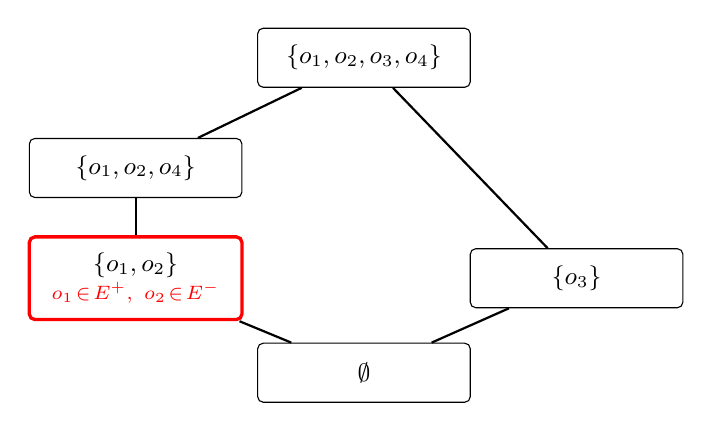
\begin{tikzpicture}[
  concept/.style={draw, rounded corners=2pt, minimum width=2.7cm, minimum height=0.75cm, font=\small, align=center},
  edge/.style={thick}
]
\node[concept] (top) at (0,4.0) {$\{o_1,o_2,o_3,o_4\}$};
\node[concept] (m1)  at (-2.9,2.6) {$\{o_1,o_2,o_4\}$};
\node[concept, draw=red, very thick, minimum height=1.05cm] (c) at (-2.9,1.2)
  {$\{o_1,o_2\}$\\[-1pt]{\scriptsize\color{red}$o_1\!\in\!\Epos,\ o_2\!\in\!\Eneg$}};
\node[concept] (m2)  at (2.7,1.2) {$\{o_3\}$};
\node[concept] (bot) at (0,0) {$\emptyset$};
\draw[edge] (top) -- (m1);
\draw[edge] (top) -- (m2);
\draw[edge] (m1) -- (c);
\draw[edge] (c) -- (bot);
\draw[edge] (bot) -- (m2);
\end{tikzpicture}%
}
\caption{A concept lattice for a context with two attributes. The positive and the negative example fall in the same
concept, so every node of the lattice above or below it contains both or neither: no hypothesis
definable in this vocabulary separates them (Theorem~\ref{thm:necessary}), and a larger budget
over the same lattice changes nothing. The only way out is adding an attribute that separates the two objects of the highlighted node.}
\label{fig:collision}
\end{figure}

\begin{theorem}[Monotonicity]\label{thm:mono}
If $\Vocab \subseteq \Vocab'$ then $\approx_{\Vocab'} \;\subseteq\; \approx_{\Vocab}$. If $p$
separates $x$ and $y$ then $x \not\approx_{\Vocab \cup \{p\}} y$.
\end{theorem}

\begin{theorem}[Capacity]\label{thm:capacity}
For a finite sample $E \subseteq \dom$, write $m = |\{\sig_{\Vocab}(x) : x \in E\}|$. The number of distinct restrictions to $E$ of
$\Vocab$-definable sets is at most $2^{m}$.
\end{theorem}

\begin{theorem}[More data does not repair a vocabulary]\label{thm:monodata}
If $\mathcal{F}_{\Vocab}(Q) = \emptyset$ then $\mathcal{F}_{\Vocab}(Q') = \emptyset$ for every query
$Q'$ whose positive set contains $\Epos$ and whose negative set contains $\Eneg$. Moreover the
candidate set can only shrink as examples are added, so additional examples can reveal an
insufficient vocabulary but never fix it.
\end{theorem}

\begin{corollary}[Rephrasing cannot separate]\label{cor:rephrase}
In the model a question is a membership test on an object, so its wording is not part of the query.
If the target is not $\Vocab$-definable and the consistent set contains two $\Indist$-equivalent
candidates, any finite number of differently worded questions leaves both live, so $\Phi \ge 2$
throughout; by Theorem~\ref{thm:mono} the set drops to $1$ only after a representation change adds a
predicate on which the candidates differ.
\end{corollary}

The diagnostic is worth stating because it inverts the usual reading. A target that survives many
rephrasings is not under-described but unrepresented: each phrasing is the same evidence about the same
signature, and the missing element is a predicate, not an example.
\begin{theorem}[Query lower bound]\label{thm:lower}
Let $\mathcal{F}$ be a family of candidate intensions pairwise distinct on $\dom$. Identifying
an element of $\mathcal{F}$ using only membership queries requires at least
$\lceil \log_2 |\mathcal{F}| \rceil$ queries.
\end{theorem}

\begin{theorem}[Covering criterion]\label{thm:cover}
If for every $x \in \Epos$ and $y \in \Eneg$ there is $p \in \Vocab$ with $p(x) \neq p(y)$, then no
class contains a positive and a negative example. Conversely, an unseparated pair is a colliding
pair, so the vocabulary suffices exactly when the chosen predicates separate every cross pair.
\end{theorem}

\section{Operators as typed transitions}\label{sec:operators}

The model of Section~\ref{sec:setting} fixes the vocabulary and lets evidence accumulate; enlarging the
vocabulary enters as a repair applied from outside. A decision procedure needs more than one kind of
step. It can generate candidates (induction, abduction, analogy), close them under rules it already
accepts (deduction, consistency filtering), change the vocabulary, buy evidence (counterexample
search, experiment), or spend budget deciding among these. Catalogued as different kinds of reasoning
they stay incomparable, so ``use the right operator'' is a slogan; one state, one measure and one type
make it checkable, and the four theorems below fix for each class what it can and cannot change.

\begin{definition}[State, live set, potential]
A \emph{state} is $s=(H,\Vocab,E,B)$: a finite family $H$ of candidate intensions, a vocabulary
$\Vocab$, evidence $E=(\Epos,\Eneg)$, and a budget $B$. Its \emph{live set} and \emph{potential} are
\[
  L(s)=\{h\in H:\ \Epos\subseteq h,\ h\cap\Eneg=\emptyset\},
  \qquad \Phi(s)=|L(s)|.
\]
A concept is \emph{decided} when $\Phi(s)=1$ and \emph{exhausted} when $\Phi(s)=0$. With $H$ the
family of all $\Vocab$-definable sets, $L(s)=\mathcal{F}_{\Vocab}(Q)$, so
Theorem~\ref{thm:necessary} says that a colliding pair forces the exhausted state for as long as the
vocabulary is unchanged.
\end{definition}

\begin{definition}[Operator, type, warrant, falsifier]
An \emph{operator} is a partial map on states with a type
$(\mathrm{rd}(o),\mathrm{wr}(o),\mathrm{dir}(o))$, where $\mathrm{rd},\mathrm{wr}\subseteq
\{H,\Vocab,E,B\}$ and $\mathrm{dir}\in\{\uparrow,\downarrow,\varnothing\}$, a
\emph{warrant}, a cost $c(o)\in\mathbb{N}$, and a \emph{falsifier}. The warrant is what makes the
output admissible --- a derivation for closure, a cover for generation, an oracle answer for evidence,
a retained partition for a representation change --- its candidates must be expressible in
the enlarged vocabulary; the falsifier is the event that voids the step. The
type answers two questions about a pair: $o_2$ is \emph{informed} by $o_1$ when
$\mathrm{rd}(o_2)\cap(\mathrm{rd}(o_1)\cup\mathrm{wr}(o_1))\neq\emptyset$, and $o_2$ is
\emph{redundant after} $o_1$ when $\mathrm{wr}(o_2)\subseteq\mathrm{wr}(o_1)$.
\end{definition}

The type, direction included, fixes the class; $\mathrm{wr}$ alone takes four values and cannot tell
generation from closure. \emph{Generation} writes $H$ by inclusion, $H\subseteq H'$:
induction, abduction, analogy. \emph{Closure} writes $H$ by filtering to the candidates consistent
with $E$: deduction and consistency checks. \emph{Representation} writes $\Vocab$, and through it $H$,
since the new atom admits candidates that were inexpressible; a relation enters as the image or
preimage of a set, a unary predicate proposed as an atom. \emph{Evidence}
writes $E$. \emph{Control} writes $B$ and selects among the others. The next four results say what
each class can do to $\Phi$.

\begin{theorem}[Generation is monotone]\label{thm:gen}
If $H\subseteq H'$ while $\Vocab$ and $E$ are unchanged, then $\Phi(H')\ge\Phi(H)$.
\end{theorem}
\begin{proof}
$L$ is monotone in $H$ and cardinality is monotone in inclusion.
\end{proof}

\begin{theorem}[Closure is idempotent]\label{thm:clos}
Let $H'=\{h\in H:\Epos\subseteq h,\ h\cap\Eneg=\emptyset\}$. Then $\Phi(H')=\Phi(H'')$, where $H''$
is obtained from $H'$ by the same closure, and every further closure step over the same evidence
leaves $\Phi$ unchanged.
\end{theorem}
\begin{proof}
$L(H')=L(H)$, and filtering an already filtered family by the same predicate changes nothing.
\end{proof}

Two consequences matter. First, \emph{thinking again is not a step}: closure is a function of $E$
alone, so repeating it re-derives the same live set --- the formal counterpart of the survey finding
that models do not correct themselves from prompted feedback alone~\cite{kamoi2024}. Second, closure
lowers $\Phi$ at most once; a run of generation and closure reaches its fixed point at the first
closure, and no later step of those two classes moves it.

\begin{theorem}[Evidence is the only strict reducer]\label{thm:ev}
If $h_2\in L(s)$ and $x\notin h_2$, then querying $x$ and receiving the answer $1$ yields
$\Phi(s')<\Phi(s)$. Consequently, with $\Vocab$ unchanged and $\Phi\ge 2$ after the first closure,
only an evidence step can lower $\Phi$.
\end{theorem}
\begin{proof}
The new live set keeps the candidates containing $x$ and drops the rest. It is a subset of $L(s)$, and
$h_2$ is dropped, so the inclusion is strict. Generation raises $\Phi$
(Theorem~\ref{thm:gen}) and closure is idempotent (Theorem~\ref{thm:clos}), so neither can be the step
that lowers it.
\end{proof}

\begin{theorem}[Recombination cannot break a collision]\label{thm:recomb}
Let $p$ be any Boolean combination of $\Vocab$, that is $p(z)=\varphi(\sig_{\Vocab}(z))$ for some
$\varphi$. If $x\Indist y$ then $p(x)=p(y)$ and $x,y$ remain indistinguishable in
$\Vocab\cup\{p\}$. Consequently, if $H$ is the family of all $\Vocab$-definable sets and the state is
exhausted, it is still exhausted after the vocabulary grows by $p$.
\end{theorem}
\begin{proof}
$\sig_{\Vocab}(x)=\sig_{\Vocab}(y)$ gives $p(x)=p(y)$ by congruence, and a predicate that agrees on a
pair cannot separate it (Theorem~\ref{thm:mono}).
\end{proof}

This is the formal content of the remark in Section~\ref{sec:exploration} that escaping an insufficient
vocabulary takes a new atom rather than a new combination: metarule composition, anti-unification
over the current predicates, and every derived feature are Boolean combinations, so they preserve
every collision.

\begin{corollary}[Alternation]\label{cor:alt}
When $H$ is the family of all $\Vocab$-definable sets and $\Phi=0$, generation and closure keep
$\Phi=0$ and evidence cannot raise it; only a representation step adding an atom outside $\Vocab$ can.
When $\Phi\ge 2$ and $\Vocab$ is fixed, only evidence can lower $\Phi$
(Theorems~\ref{thm:gen}--\ref{thm:ev}). Hence deciding a concept requires alternating representation
change with evidence acquisition, and no single class of operator suffices.
\end{corollary}
\begin{proof}
At $\Phi=0$ every $\Vocab$-definable candidate is inconsistent with $E$; generation inside $\Vocab$
adds only such candidates, closure removes candidates, and evidence adds constraints, so the live set
stays empty. At $\Phi\ge2$ the claim is Theorem~\ref{thm:ev} with Theorems~\ref{thm:gen}
and~\ref{thm:clos}. The two halves are Theorems~\ref{thm:necessary} and~\ref{thm:lower} read as
statements about one measure.
\end{proof}

Two terms usually applied here are second order: meta-learning and inductive bias change the
generation operator or $H$, not the state; compositional generalization is a property of the language
the generator emits. Neither is a class of its own, and neither is validated by $\Phi$ --- the live set
is a count, not a preference. The typing says only where they must act (representation,
Corollary~\ref{cor:alt}) and that they cannot supply evidence.

Read competitively, the live set is what survives: a population, an answer that can kill part of it,
and no hope that re-ranking changes the verdict.

Control moves no potential. Its entire contribution is to avoid redundant steps: a closure after the
first is redundant (Theorem~\ref{thm:clos}), a generation that adds no consistent candidate
cannot change $\Phi$, and an evidence step that is uniform on the live set only constrains later
candidates. This bounds
what scheduling can buy. Between two runs that reach the same state, the cost difference is the cost
of the redundant steps in the dearer one, and by Theorem~\ref{thm:clos} no schedule can make closure
cheaper than once. The measurement in Section~\ref{sec:experiments} is the same statement: query ordering
moved total cost within $\pm 6\%$ while $r/q$ spanned a factor of $45$, because informative questions
differ in how much they split the live set, and the number of questions needed to decide lies between
the counting bound of Theorem~\ref{thm:lower} and the trivial bound $\Phi-1$. On uniform query costs
with eight live hypotheses, selecting by split size needs $3.11$ queries against $3.50$ for a random
order and $3.60$ for a fixed one, a gap of about four tenths of a query, which is what
second order means here. When a single atom suffices, coverage ranks it first, and then the score is
the criterion rather than a proxy: by Theorem~\ref{thm:cover} such an atom separates every colliding
pair. Greedy composition extends past the single-atom case: with two atoms required, it succeeds
within a budget of two, a random order rarely, a fixed order not in our runs.

It does not say which candidate to generate, or whether the survivor is the user's concept. It says
that no sequence of the other four classes changes the verdict, so adding operators to a fixed
vocabulary, or re-deciding closure, cannot converge; Section~\ref{sec:exploration} alternates expansion,
which changes $\Vocab$, with queries, which change $E$.

\section{Exploration procedure}\label{sec:exploration}

State: a vocabulary $\Vocab$ and the candidate set $\mathcal{F}$. Loop:
\begin{enumerate}
  \item if $\mathcal{F} = \emptyset$, Theorem~\ref{thm:necessary} certifies that the vocabulary is
        insufficient; enter expansion;
  \item if $|\mathcal{F}| = 1$, stop;
  \item otherwise ask the oracle about a representative of an unresolved class; as Section~\ref{sec:experiments} shows, which
        representative is chosen barely matters;
  \item on expansion, a candidate predicate \emph{covers} the cross pairs $(x,y) \in \Epos \times
        \Eneg$ that it separates; by Theorem~\ref{thm:cover} the vocabulary becomes sufficient once
        the covers exhaust the cross product, so proposal is a set-cover problem and greedy is an
        $H_{|\Epos||\Eneg|}$ approximation. In synthetic covering experiments ($3\times3$ pairs,
        ten random candidates) greedy needs $2.10 \pm 0.06$ predicates on average against
        $1.85 \pm 0.06$ for the optimum and $4.28 \pm 0.09$ for a random order (five seeds).
        Metarule-style combination is not a way out: every
        candidate built from the current predicates is again $\Vocab$-definable, so on a run with
        whose only predicate halved its argument, the derived candidate pool contained one predicate that
        separated none of the four colliding pairs. Escaping an insufficient vocabulary requires a
        new atom, not a new combination.
\end{enumerate}
The three roles---proposal, selection, adjudication---are kept separate so that they do not
share a single source of error. Under a noisy oracle one rule is added: a class counts as decided
only when every member that received any vote has reached the margin $\theta$, and a conflict is
re-confirmed before a predicate is proposed; $\theta = 3$ suffices for per-answer error
$\varepsilon \le 0.1$. A small Rust library mirrors Theorems~\ref{thm:necessary}, \ref{thm:capacity}, \ref{thm:monodata}
and, for the operators of Section~\ref{sec:operators}, Theorems~\ref{thm:gen}--\ref{thm:recomb}, including
a probe operator that validates an inherited class label and on which the stopping rule depends;
Its scheduling comparison reports the cost difference as the number of skipped
steps.

\section{Empirical results}\label{sec:experiments}

\textbf{Domain A (synthetic formal contexts).} Twelve objects, eight attributes, and a target
concept defined by a ninth attribute absent from the initial vocabulary. In $300/300$ instances
no concept definable in the initial vocabulary is consistent with the examples, confirming
Theorem~\ref{thm:necessary} empirically. Under a bounded-conjunction class, identifying the target
takes $2.01 \pm 0.06$ queries on average with expected information gain, $1.91 \pm 0.07$ with
uniformly random \emph{informative} questions, and $6.14 \pm 0.23$ with naive random questions
(five seeds, 150 instances each). The improvement therefore comes from
not asking redundant questions, not from choosing cleverly: every informative question is worth
the same bit; if anything, information gain is slightly worse than picking informative questions
at random.
An Occam prior $p(S)\propto 2^{-|S|}$~\cite{grunwald2019} separates the policies only slightly
($1.63$ vs $1.87$). This negative result moves the optimisation target from object selection to the
vocabulary-level decision of when to stop asking and what to propose.

\textbf{More examples make it worse, not better.} Theorem~\ref{thm:monodata} says an insufficient
vocabulary cannot be repaired by additional examples. Sampling $k$ examples from the same
instances, the probability that no consistent concept exists in the initial vocabulary rises from
$2.5\%$ at $k=1$ to $29.5\%$ at $k=4$ and $98.7\%$ at $k=10$: examples expose the mismatch instead
of resolving it.

\textbf{Cost accounting.} Take object queries to cost $1$ (all costs are in query units) and a predicate proposal to cost
$r \in \{5, 20, 100\}$ with hit rate $q$. Total cost is governed by the ratio $r/q$: across the
grid it spans a factor of about $45$, while the choice between asking first and proposing first stays
within $\pm 6\%$ and changes sign. Scheduling is a second-order decision; the proposer's hit rate
is first-order. This is why the procedure above spends no machinery on query ordering.

The same law holds in the executable loop rather than only in the cost model. With $r = 20$, a
proposer that is right with probability $q$, and $7.6$ query rounds (independent of $q$), measured
total cost is $27.6$, $49.4$, $88.9$ and $162.7$ for $q = 1, \tfrac12, \tfrac14, \tfrac18$ ---
close to $r/q + 7.6$: proposal counts $1.00$, $2.09$, $4.07$, $7.75$ leave a residual within sampling
noise, and wasted proposals grow as $1/q-1$.

The accounting is written for an agent, not for a human expert. Queries are answered by programs
or by batched model calls and cost one round each; proposals cost tokens, validation, and sometimes
a failed experiment. Moving from per-query to per-round accounting only strengthens the conclusion:
rounds are cheaper than proposals, so $r/q$ dominates even more.

\textbf{Cheap proposals.} Suppose the proposer becomes cheap, $r \to 0$. The law $r/q + 7.6$ then tends
to $7.6$, the query rounds, and stops: cheap proposals cancel the proposal term and leave the evidence
term. What they buy is a vocabulary in which those queries are not wasted, since by
Theorem~\ref{thm:monodata} queries spent under an insufficient vocabulary are unrecoverable. Measured:
with $k$ candidate vocabularies, exactly one containing the target predicate, a baseline that draws one
member at random succeeds $0.250$ at $k=5$ and the portfolio $0.955$, paying $1.53$ queries to eliminate
each wrong candidate (disagreement sampling, $200$ trials). The portfolio is never wrong; it fails only
by conflict, which rises from $0.025$ at $k=3$ to $0.110$ at $k=10$, so success peaks at $k=3$ ($0.975$)
and falls back at $k=10$ ($0.890$). Cheap proposals remove the $1/k$ lottery of a single guess, not the
queries; the useful size is where the failure prevented outweighs the conflict added.
\textbf{Domain C (code invariants).} Twelve test inputs for an interval-merging function; the hidden
invariant is that the output is shorter than the input. Predicates are executable features of the
input; the oracle runs the function. With six features in the vocabulary the two seed examples
collide, the state is \emph{exhausted}, and no number of further examples can help. Three
plausible decoy predicates (all-positive, length at most two, small adjacent gap) take the same
value on the colliding pair and therefore leave the state unchanged: a wrong predicate is not
weakly useful, it is exactly useless. The fourth proposal (``contains an overlapping or touching
pair'') leaves the exhausted state, after which eight membership queries recover the extension
exactly. At a proposal cost of $20$ this is $88$ versus $28$ for a proposer that is right the first
time: the whole difference is proposal quality. Ordering recovers the second figure without a better
proposer: scoring the same four candidates by separated colliding pairs puts the sufficient one first,
so the cost is $28$ again, against $88$ in file order and $57.2$ at random. A target that needs two
predicates exposes the stopping rule. When a class label is inherited by its members, the loop can
report a unique consistent concept that is wrong: it stops after one proposal and the extension
differs from the target. Probing one unasked member of each multi-member class makes the state
exhausted again and recovers the right extension in two proposals, at a cost of $3$ extra queries in
the one-atom case ($28 \to 31$) and $51$ against $111$ in file order in the two-atom case. The same scoring drives a
proxy proposer interface
that sends the colliding pairs to a model and scores the returned predicates by how many pairs they
separate ($4/4$, $2/4$, $0/4$, $2/4$ for four candidates); the scoring is mechanical, the response
in our run was supplied by hand. Scoring against the hidden extension separates sound-but-narrow
candidates from wrong ones: two candidates both cover $2/4$ pairs, yet one has recall $0.67$ and the
other $0.33$, while one candidate has precision $0.67$ and another $1.00$ on only a third of the
target. Only the candidate with precision and recall both $1.00$ should enter the vocabulary. In deployment the
check can enforce soundness only: predictions confirmed by the oracle reject a candidate whose
predictions fail, but two of the four candidates are sound and still incomplete (precision $1.00$,
recall $0.33$ and $0.67$), so completeness has to come from further queries rather than from the
prediction test. A reverse probe does this: a second party names an object the candidate excludes,
the oracle confirms it positive, and the candidate is shown to be incomplete. In our run the probe kills
exactly the three incomplete candidates and leaves the correct one standing, using only oracle
answers. Confirmed counterexamples are kept in a ledger, so a later proposal that excludes any of
them is rejected without further probing; in our second round a freshly proposed candidate that
repeats an earlier mistake is caught this way with no probe of its own. The ledger serves two
distinct roles: a candidate may be rejected as a \emph{definition} of $S$ and still remain a
legitimate element of the set-cover composition of Theorem~\ref{thm:cover} if it is sound, and a
candidate that supplies no confirmed prediction is accepted in neither role. The ledger is a
mutable knowledge base rather than an append-only set: an entry can be retracted when the oracle
answer behind it is later found wrong, or amended when it recorded the wrong object, and each
change carries a reason and a timestamp. Entries also record the target concept they were confirmed
against: when the target is redefined they are suspended rather than deleted, and only revalidated
entries judge again, so a change of goal neither loses evidence nor silently keeps stale evidence. Each entry also
records the oracle answer that justified it --- object, answer, source and, when the oracle is
noisy, the vote counts -- so that a judgment can always be traced back to the evidence it rests on. Reliability is part of
the evidence: an entry whose oracle is a model rather than a test is weighted below the hard
threshold and only raises a soft flag, so a noisy source is recorded without being allowed to veto
a candidate on its own. Independent weak pieces of evidence about the same object combine by
noisy-OR, $1-\prod_i(1-r_i)$: in our run two half-reliable sources reach $0.75$ and stay soft,
three reach $0.88$ and become hard, and the merged entry keeps the identifiers of its constituents. Evidence also carries direction:
when a case has both positive and negative support above threshold its truth is treated as unknown,
it stops blocking any candidate, and it is queued for re-query, since noisy-OR would otherwise turn
disagreement into apparent certainty. The queue is ordered by the gap between the two sides and
carries a suggested number of further confirmations, and a conflict requires the two sides to be
comparable ($\min \ge 0.7\max$): overwhelming evidence is not cancelled by a weak dissent. Re-queries are planned the same way as
proposals: conflicted objects that share an equivalence class need one query rather than one each,
so the covering argument of Theorem~\ref{thm:cover} applies to the conflict set as well (three
conflicts needed two queries in our run). The plan also checks purity: a class known to contain both
a confirmed positive and a confirmed negative is impure, and each conflicted member is then asked
separately; a class with no such evidence gets one representative, with the stated risk that the
answer may not transfer to its other members. For such a class the plan compares expected costs:
one representative costs $1+(1-p)(c-1)R$ when a wrong class label forces $c-1$ relabellings at
rework cost $R$, while asking every conflicted member costs $c$; the choice flips from one query at
$R=1$ to all of them at $R=3$ in our run. The purity prior is not hand-set either: it is estimated
from the ledger by Laplace smoothing over classes that carry at least two confirmed labels ($1$ of
$1$ impure gives $p=0.67$ in our run, and the estimate is printed with the plan), so the one free
parameter of the cost comparison is tied to recorded evidence. The last parameter, the rework cost
$R$, is estimated the same way: eleven repair actions over nine repaired entries give $R=1.22$ in
our ledger, and the plan then asks one representative where a hand-set $R=3$ would have asked both. The trace is kept with the artifacts.

\textbf{Domain B (mathematics, Lean oracle).} Twenty-one integers in $[11,31]$; the hidden concept is
primality. A Lean file with no Mathlib imports computes the truth table and, inside Lean, proves
that on this interval primality coincides with coprimality to $30$; the Python loop then consumes
that table. One Lean invocation costs $2.5$\,s and answers every query at once, whereas answering
the five queries individually would cost $12.6$\,s. The loop behaves exactly as in domain C: the
only decoy that agrees on the colliding pair changes nothing, and the concept becomes definable
only once the right predicate arrives.

\begin{figure}[t]
\centering
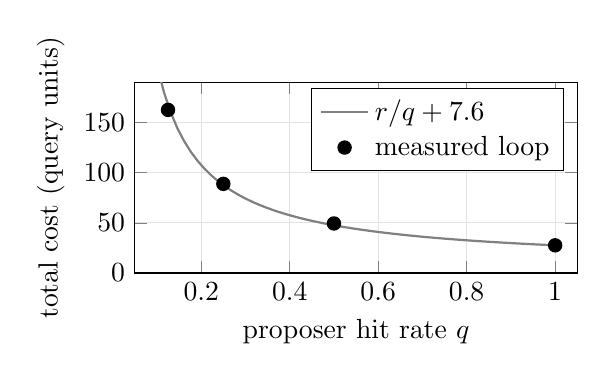
\begin{tikzpicture}
\begin{axis}[
  width=7.2cm, height=4.0cm,
  xlabel={proposer hit rate $q$}, ylabel={total cost (query units)},
  xmin=0.05, xmax=1.05, ymin=0, ymax=190,
  legend pos=north east, legend cell align=left,
  grid=major, grid style={gray!22},
]
\addplot[domain=0.1:1.0, samples=60, thick, gray] {20/x + 7.6};
\addlegendentry{$r/q + 7.6$}
\addplot[only marks, mark=*, mark size=2.2pt, thick] coordinates {
  (0.125,162.7) (0.25,88.9) (0.5,49.4) (1.0,27.6)
};
\addlegendentry{measured loop}
\end{axis}
\end{tikzpicture}\hfill
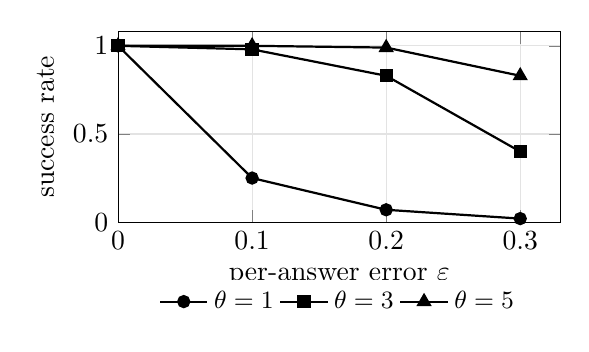
\begin{tikzpicture}
\begin{axis}[
  width=7.2cm, height=4.0cm,
  xlabel={per-answer error $\varepsilon$}, ylabel={success rate},
  xmin=0, xmax=0.33, ymin=0, ymax=1.08,
  legend style={at={(0.5,-0.30)}, anchor=north, legend columns=3, draw=none, font=\small},
  grid=major, grid style={gray!22},
]
\addplot[thick, mark=*, mark size=2pt] coordinates {(0,1.00)(0.1,0.25)(0.2,0.07)(0.3,0.02)};
\addlegendentry{$\theta=1$}
\addplot[thick, mark=square*, mark size=2pt] coordinates {(0,1.00)(0.1,0.98)(0.2,0.83)(0.3,0.40)};
\addlegendentry{$\theta=3$}
\addplot[thick, mark=triangle*, mark size=2.4pt] coordinates {(0,1.00)(0.1,1.00)(0.2,0.99)(0.3,0.83)};
\addlegendentry{$\theta=5$}
\end{axis}
\end{tikzpicture}
\caption{Left: total cost against the proposer's hit rate; the measured points follow $r/q+7.6$.
Right: end-to-end success against oracle error for three vote margins. Raising $\theta$ buys accuracy
with rounds, and $\theta=1$ collapses; the gap between $\theta=3$ and $\theta=5$ opens only beyond
$\varepsilon \approx 0.2$.}
\label{fig:curves}
\end{figure}

\section{Limitations}

\textbf{Noise.} The formal results assume an oracle that answers correctly and consistently; the
procedure tolerates errors only up to about $\varepsilon = 0.2$, by requiring vote margins. Noise
turns the necessity criterion into a statistical one: the trigger becomes ``no concept explains the
answers at confidence $\delta$'', and the capacity bound has to be read as a sample-complexity
statement. In synthetic runs with per-answer error $\varepsilon$ and majority voting over $m$
repeated queries, $m=5$ keeps the false-trigger rate at or below $0.5\%$ for $\varepsilon \le 0.2$
and removes missed detections, while $\varepsilon = 0.3$ leaves both near $8\%$: repetition buys
reliability, but not without limit.

\textbf{Decidable membership only.} Predicates such as ``is a natural kind'' have no membership
function, so the framework says nothing about them. This is a real restriction, not a presentational
one: the whole point of the criterion is that it can be checked.

\textbf{Single-predicate growth.} The procedure proposes one predicate at a time. Batch growth needs
a criterion for which subset to request, and the obvious candidates (marginal information gain) are
not obviously submodular.

\textbf{Extensional equivalence.} Two different predicates may have the same extension; the capacity
count then overstates the number of distinguishable concepts. Quotienting by extensional equality is
easy to state and annoying to implement in the presence of partial information.

\textbf{Scope of the evidence.} The empirical results are on synthetic contexts and one small code
domain; no language-model proposer is in the loop yet. The claim defended here is the necessity
criterion and the shape of the procedure, not the quality of any particular proposer.

\textbf{One measure, not truth.} The potential counts live hypotheses. It is blind to whether the
surviving hypothesis is the concept the user has in mind, and blind to description length, so a
generation step that raises $\Phi$ can still be a good step under a minimum description length reading. A second measure
would refine the typing rather than contradict it; we do not have the corresponding theorems.

\textbf{Implementation.} The reference kernel handles at most 64 objects (single machine word) and
does not deduplicate extensionally equivalent predicates.

\appendix

\section{Mechanized statements}

13 Lean~4~\cite{lean4} declarations, over Mathlib~\cite{mathlib}, carry Theorems~\ref{thm:char}--\ref{thm:recomb}: one
characterization, the necessity statement, the two monotonicity lemmas, the counting form of the
capacity bound, the no-repair statement, the query lower bound, the covering criterion, and one
statement per operator class, recombination split into two. The development compiles with no admitted
goal and no warnings, in about 25\,s once Mathlib is warm, and the build fails on a warning, so the
machine check is enforced by the build rather than reported here. Two signature lemmas and the weak
counting form support those proofs and are not counted. The operator statements are phrased over the
live set and the potential of Section~\ref{sec:operators}. The corollary of Section~\ref{sec:setting} on rephrasing
and the corollary of Section~\ref{sec:operators} on alternation are paper-level consequences and are not
separately mechanized.

Every number quoted in Section~\ref{sec:experiments} is re-compared by an automated gate against a fresh run
of the experiments and of the kernel, so a number that drifts fails the build. The synthetic
experiments use only the Python standard library; domain~B requires a Lean toolchain; domain~C runs the
function it characterizes and never reads the invariant.
\begin{thebibliography}{9}
\small
\bibitem{cropper2021} A.~Cropper, S.~Duman\v{c}i\'c, and R.~Evans.
  Inductive logic programming at 30. \emph{Machine Learning}, 2021.
\bibitem{kemp2010} C.~Kemp, N.~D.~Goodman, and J.~B.~Tenenbaum.
  A probabilistic model of theory formation. \emph{Cognition}, 114:165--196, 2010.
\bibitem{perfors2011} A.~Perfors, J.~B.~Tenenbaum, T.~L.~Griffiths, and F.~Xu.
  A tutorial introduction to Bayesian models of cognitive development. \emph{Cognition}, 2011.
\bibitem{friston2026} K.~Friston, L.~Da Costa, A.~Tschantz, C.~Heins, C.~L.~Buckley, T.~Verbelen,
  and T.~Parr. Active inference and artificial reasoning. \emph{Nature Communications}, 2026.
\bibitem{kamoi2024} R.~Kamoi, Y.~Zhang, N.~Zhang, J.~Han, and R.~Zhang.
  When can LLMs actually correct their own mistakes? A critical survey of self-correction of LLMs.
  \emph{TACL}, 2024.
\bibitem{kemp2008} C.~Kemp and J.~B.~Tenenbaum. The discovery of structural form.
  \emph{PNAS}, 2008.
\bibitem{ellis2020} K.~Ellis et al. DreamCoder: growing generalizable, interpretable knowledge
  with wake--sleep Bayesian program learning. 2020.
\bibitem{falkenhainer1989} B.~Falkenhainer, K.~D.~Forbus, and D.~Gentner.
  The structure-mapping engine. \emph{Artificial Intelligence}, 1989.
\bibitem{clarke2000} E.~Clarke et al. Counterexample-guided abstraction refinement. 2000.
\bibitem{russell1991} S.~Russell and E.~Wefald. Principles of metareasoning.
  \emph{Artificial Intelligence}, 49(1--3):361--395, 1991.
\bibitem{grunwald2019} P.~Gr\"unwald and J.~Roos. Minimum description length revisited. 2019.
\bibitem{lean4}
  L.~de Moura and S.~Ullrich. The Lean~4 theorem prover and programming language.
  \emph{CADE}, 2021.
\bibitem{mathlib}
  The Mathlib community. The Lean mathematical library. \emph{CPP}, 2020.
\bibitem{ganter1999} B.~Ganter and R.~Wille. \emph{Formal Concept Analysis: Mathematical
  Foundations}. Springer, 1999.
\normalsize
\end{thebibliography}


\vspace{1em}
\noindent\small\textit{License.} This text is released under the Creative Commons Attribution 4.0
International license (CC BY 4.0).
\end{document}
































